\section{Strategized Locking}

The Strategized Locking design pattern parameterizes synchronization mechanisms that protect a component's critical sections from concurrent access

\subsection*{Kontext}

Eine Applikation welche effizient auf verschiedenen Concurrency-Architekturen laufen muss (z.B. Single-Threaded und Multi-Threaded)

\subsection*{Problem}

Unterschiedliche Applikationen könnten unterschiedliche Synchronisations-Strategien (Mutex, Reader/Writer lock, Semaphore) verwenden/erfordern. Es sollte daher möglich sein, den Synchronisations-Mechanismus ohne neuschreiben der Funktionalität auszutauschen.

\subsection*{Lösung}

\begin{figure}[H]
	\centering
	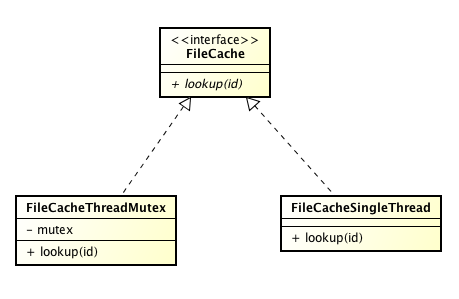
\includegraphics[width=12cm]{content/posa2/strategized-locking/images/Screen_Shot_2013-05-07.png}
	\caption{Strategized Locking Class Diagram}
\end{figure}

Um z.B. eine Single-Threaded Applikation so schnell wie möglich zu machen, kann ein Null-Objekt als Lock verwendet werden.

\subsection*{Vorteile}

\begin{itemize}
	\item Flexibilität und Anpassbarkeit wird erhöht
	\item Weniger Aufwand für die Wartung der Komponenten
	\item Wiederverwendbarkeit verbessert
\end{itemize}

\subsection*{Nachteile}

\begin{itemize}
	\item Obtrusive Locking: Wenn templates für das Locking verwendet werden, wird die Locking Strategie dem Applikations-Code überlassen. Obwohl das Design flexibel ist, kann dies auch ein Nachteil sein, insbesondere wenn Compiler Templates nicht gut unterstützen.
	\item Over-Engineering: Dieses Pattern kann z.T. zuviel Flexibilität zur Verfügung stellen.
\end{itemize}

